\documentclass[aspectratio=169,xcolor=table]{beamer}
%aspcetratio >> 1610 169 149 54 43 32
%The themes:
%\usetheme[style=classic]{mharvellous}
%\usetheme[style=dark]{mharvellous}
%\usetheme[style=mracula]{mharvellous}
\usetheme[style=default]{mharvellous}
%*--------------------------------------------------
%\usepackage{helvet}
%*--------------------------------------------------
\usepackage{bibunits}  
%\setbeamertemplate{bibliography item}{[\theenumiv]}
\setbeamertemplate{bibliography item}{\insertbiblabel}
\defaultbibliography{bibliography}
%\defaultbibliographystyle{IEEEtran}
%\defaultbibliographystyle{amsalpha}
\defaultbibliographystyle{abntex2-alf}
%\bibliography{bibliography}
%\usepackage[backend=biber,style=alphabetic,citestyle=authoryear]{biblatex}
% \addbibresource{bibliography.bib}
%\usepackage{natbib}
\usepackage{bibentry}
%*--------------------------------------------------
\usepackage{lipsum}
\usepackage{epigraph}
\usepackage{graphicx}
\usepackage{multirow}
%\usepackage{enumitem}
\usepackage{array}
%\usepackage{multimedia}
\usepackage{media9}
%\usepackage{pdfpc-movie}
\usepackage{circledsteps}
\usepackage{listings}
\usepackage[normalem]{ulem}
%\usepackage{Sweave}
%\usepackage{xkeyval}
%\usepackage{palatino}
%\usepackage{pgfpages}
\usepackage{float}
%*--------------------------------------------------
\usepackage[timeinterval=1]{tdclock}
%\usepackage[font=Times,timeinterval=1, timeduration=200,resetatpages=all]{tdclock}
%\usepackage[font=Times,timeinterval=10, timeduration=2.0, timedeath=0, fillcolorwarningsecond=white!60!yellow,timewarningfirst=50,timewarningsecond=80,resetatpages=2]{tdclock}
%*--------------------------------------------------
\usepackage{url}
\usepackage{tabularx,booktabs}
\usepackage{threeparttable}
\usepackage[absolute, overlay]{textpos}
%*--------------------------------------------------
\usepackage{framed, color}
\usepackage[tikz]{bclogo}
\usepackage{spot}
\setspotlightcolor{red!50}
% %\setspotlightstyle{star, fill=red!50}
% %\setspotlightstyle{star points=7}
\usepackage{color,soul}
%\usepackage{xcolor}
\usepackage{tcolorbox}
\usepackage{xcolor}
\usepackage[export]{adjustbox}
\usepackage{verbatim}
\usetikzlibrary{trees,shapes,arrows}
\usepackage{fancyvrb}
\usepackage{float}
%*--------------------------------------------------
\usepackage{amsmath}
\usepackage{xfrac}
\usepackage{units}
\usepackage{ulem}
%*-------------------------------------------------------------------------------
%\newcolumntype{C}[1]{>{\centering\arraybackslash}m{#1}}
\newcolumntype{L}[1]{>{\raggedright\let\newline\\\arraybackslash\hspace{0pt}}m{#1}}
\newcolumntype{C}[1]{>{\centering\let\newline\\\arraybackslash\hspace{0pt}}m{#1}}
\newcolumntype{R}[1]{>{\raggedleft\let\newline\\\arraybackslash\hspace{0pt}}m{#1}}
%*-------------------------------------------------------------------------------
%\pgfpagesuselayout{2 on 1}[a4paper,border shrink=5mm]
%\setbeamertemplate{note page}[plain]
%\setbeameroption{show notes on second screen=bottom}
%*-------------------------------------------------------------------------------
\setbeameroption{hide notes}
%\setbeameroption{show only notes}
%\setbeameroption{show notes on second screen=right}
\setbeamertemplate{note page}{\pagecolor{yellow!5}\insertnote}
%*-------------------------------------------------------------------------------

%*-------------------------------------------------------------------------------
\title              {Título}
\subtitle           {Subtítulo}
\author             {Nome Sobrenome}
\email              {nome@site.com}
\advisor            {Orientador: Marco A. dos Reis}
\institute          {Robótica e Sistemas Autônomos, Senai Cimatec}
\date               {Mês de 202x}
% \ulogo        		{Template/logosenaicimatecnegativo}
% \ulogof             {Template/logosenaicimatec2020}
% \ulogoo        		{Template/rosa-logo}
% \ulistelement    	{Template/bullet-white}

%*-------------------------------------------------------------------------------
\graphicspath{{Source/pictures/}}
%*-------------------------------------------------------------------------------
\totalNoSlidesDisabled % To turn off the total number of slides in the footer. Comment this if you want the total number of slides in the footer
%*-------------------------------------------------------------------------------
\begin{document}
%*----------- COVER -------------------------------------------------------------
 \begin{frame}[t,plain]
%*----------- sound--------------------------------
    \includemedia[
        %width=1ex,
        %height=1ex,
        %activate=pageopen, 
        activate=onclick,
        deactivate=onclick,
        %passcontext,
        transparent,
        addresource=./Source/sounds/hip-hop.mp3,
        flashvars={
                    source=./Source/sounds/hip-hop.mp3
                    %&autoPlay=true
                    &autoRewind=true
                    &Play=2s
                    &repeat=always
                    %&Loop=true
        }
    ]
    {}{VPlayer.swf}
%*----------- start-page--------------------------
    \titlepage
    %*----------- notes-------------------------------
    \note[item]{Notes can help you to remember important information. Turn on the notes option.}
\end{frame}
%-
%*----------- SECTIONS ----------------------------------------------------------
%*----------- SLIDE -------------------------------------------------------------
\begin{frame}[t]{Introdução} 
    \transdissolve[duration=0.5]
    AUV (Autnomous Underwater Vehicle) é um veiculo subaquático autônomo, o qual não é conctado por cabos 
    a um operador e não é não tripulado.
    % COLOCAR AQUI DUAS IMAGENS DE AUVS E NA HORA FALAR SOBRE OS DIFERENTES TAMANHOS 
    % E COMO OPERAM

   % \newline
    \begin{columns}[t]
        \column{.05\linewidth}
        
        \column{.4\linewidth}
        \begin{figure}
            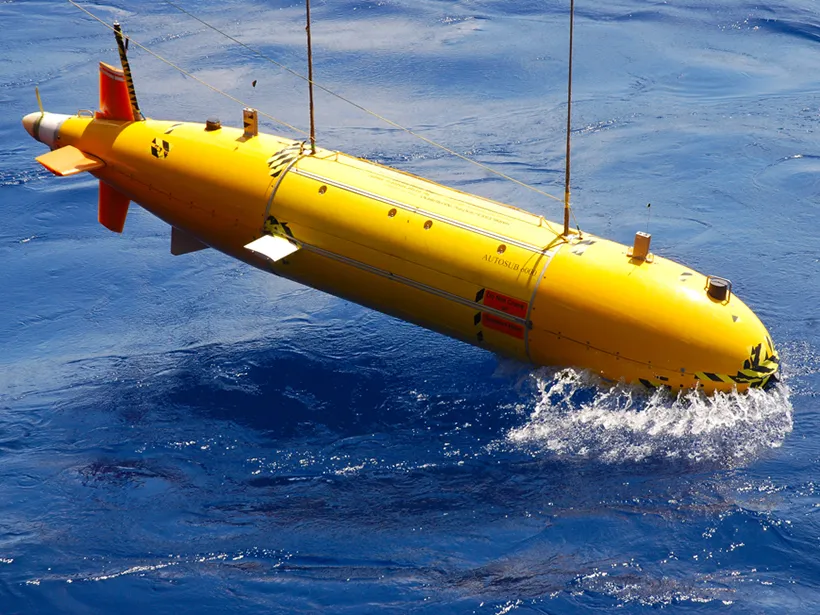
\includegraphics[height = 3.38cm, width=0.8\textwidth]{AUV_2.png}%4.3 metros de comprimento
            \caption{\nocite{REMUS6001:online}}
        \end{figure}
        
        \column{.6\linewidth}
        \begin{figure}
           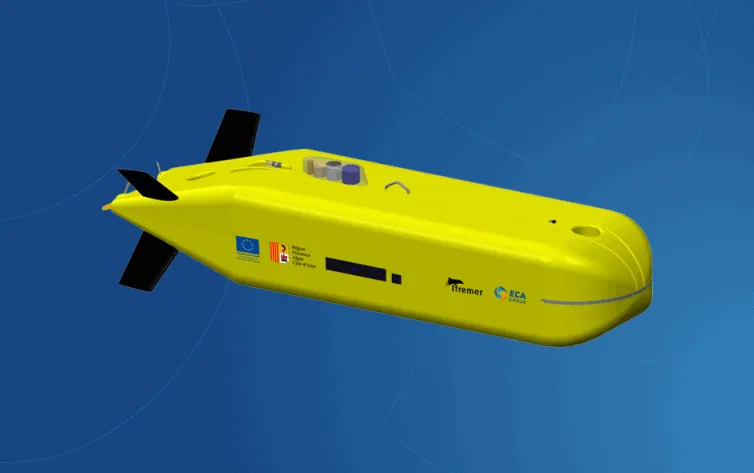
\includegraphics[height = 3.38cm, width=0.6\textwidth]{auv-3.png}%45.7cm de comprimento
            \caption{\nocite{BlueROV210:online}}
        \end{figure}
        
    \end{columns}

%*----------- notes
    \note[item]{Notes can help you to remember important information. Turn on the notes option.}
\end{frame}
%-
%*----------- SLIDE -------------------------------------------------------------
\begin{frame}[c]{Mapa Conceitual}
    %\transboxin[duration=1,direction=30]
        \begin{figure}
        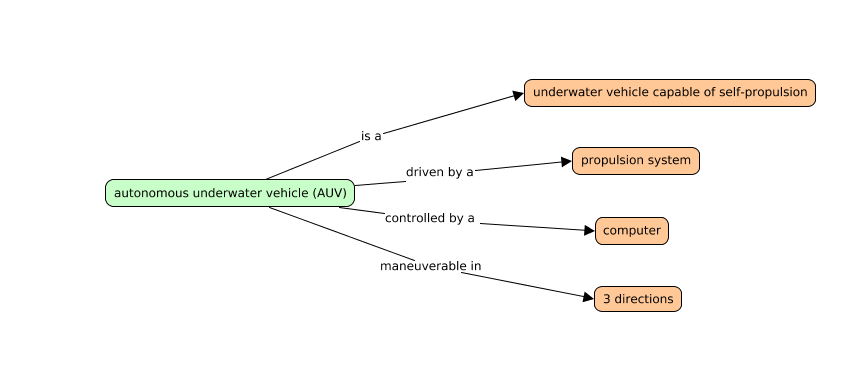
\includegraphics[width=1.1\textwidth]{mapa1modi.png}
    \end{figure}
%*----------- notes
    \note[item]{Notes can help you to remember important information. Turn on the notes option.}
\end{frame}
%-
%*----------- SLIDE -------------------------------------------------------------
\begin{frame}[c]{Mapa Conceitual}
    %\transboxin[duration=1,direction=30]
        \begin{figure}
        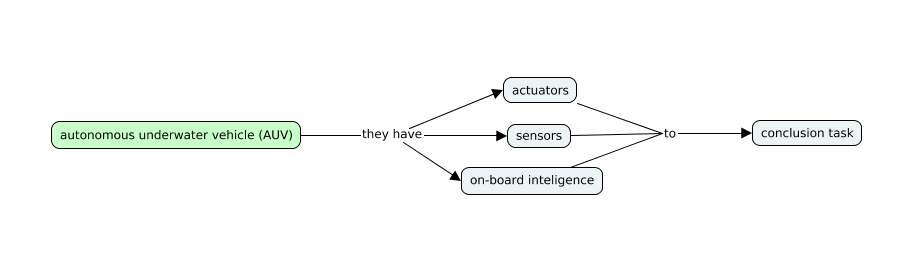
\includegraphics[width=1.1\textwidth]{mapa2modi.png}
    \end{figure}
%*----------- notes
    \note[item]{Notes can help you to remember important information. Turn on the notes option.}
\end{frame}
%-
%*----------- SLIDE -------------------------------------------------------------
\begin{frame}[c]{Mapa Conceitual}
    %\transboxin[duration=1,direction=30]
        \begin{figure}
        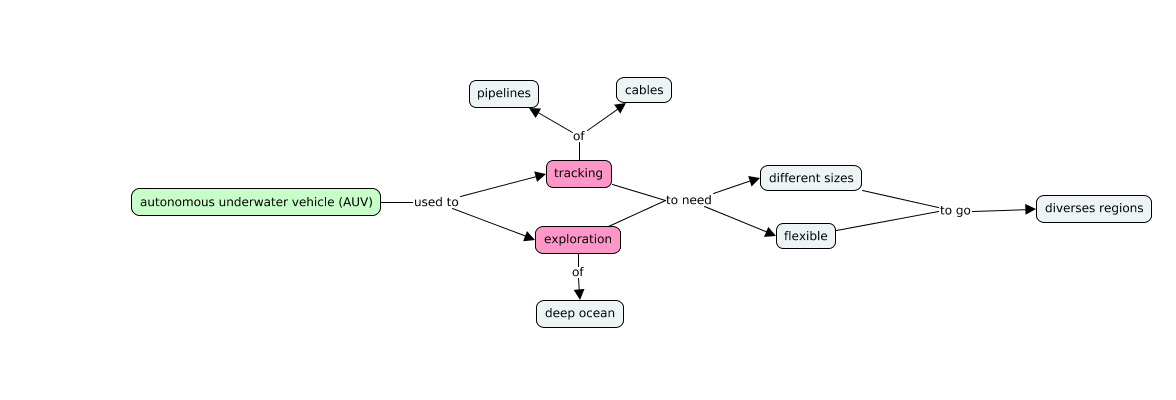
\includegraphics[width=1\textwidth]{mapa3modi.png}
    \end{figure}
%*----------- notes
    \note[item]{Notes can help you to remember important information. Turn on the notes option.}
\end{frame}
%-

%*----------- SLIDE -------------------------------------------------------------
\begin{frame}[t]{Introdução}
    \transboxout[duration=0.5]
    \framesubtitle{História}
    \begin{columns}
        \column{.1\textwidth}
        \column{.4\textwidth}
        
               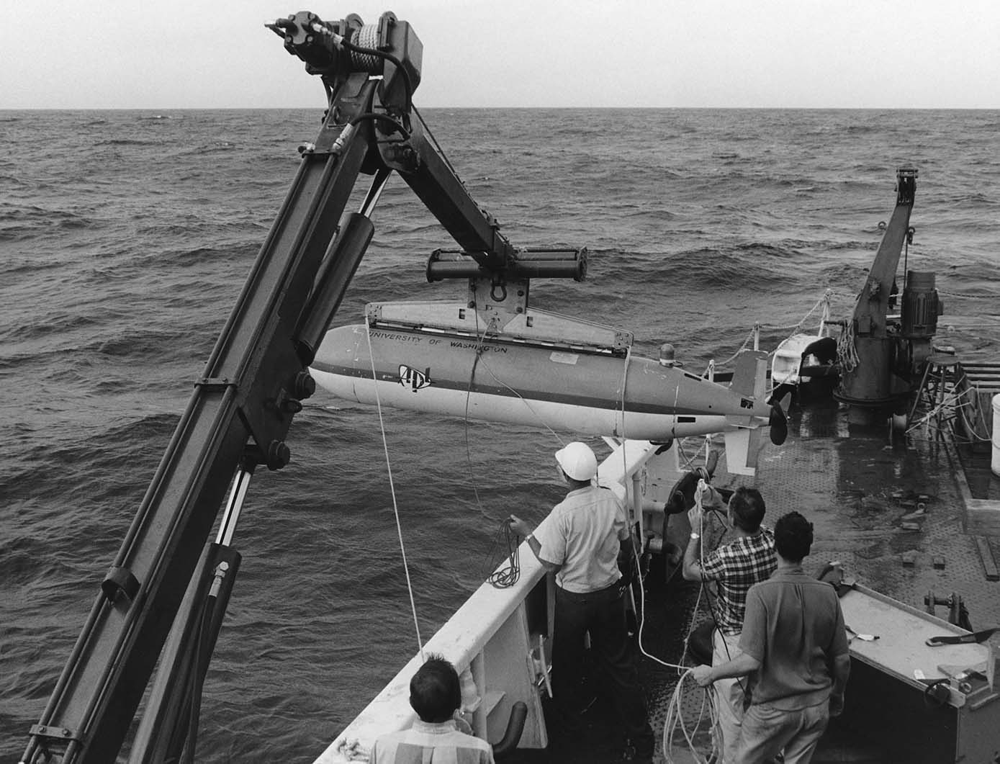
\includegraphics[width=1\textwidth]{spurv.png}
    
        \column{.4\textwidth}
            \begin{itemize}
               \item O primeiro torpedo foi enviado por Whintehead (1866)
               \item Veículo de pesquisa subaquática de propósito especial (1957)
            \end{itemize}
    \end{columns}
 %*----------- notes
    \note[item]{Notes can help you to remember important information. Turn on the notes option.}
\end{frame}
%-
%*----------- SLIDE -------------------------------------------------------------
\begin{frame}[c]{Mapa Conceitual}
    %\transboxin[duration=1,direction=30]
        \begin{figure}
        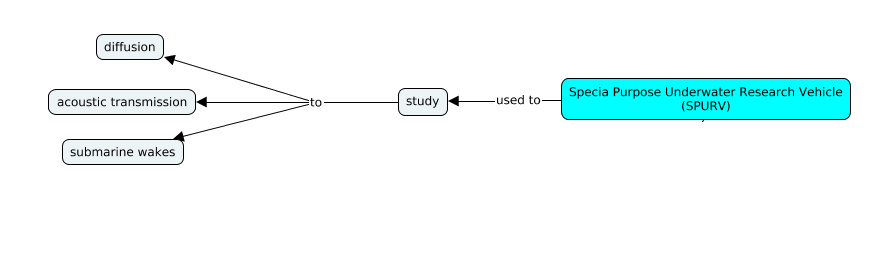
\includegraphics[width=1.1\textwidth]{mapa5modi.png}
    \end{figure}
%*----------- notes
    \note[item]{Notes can help you to remember important information. Turn on the notes option.}
\end{frame}
%-
%*----------- SLIDE -------------------------------------------------------------
\begin{frame}[c]{Mapa Conceitual}
    %\transboxin[duration=1,direction=30]
        \begin{figure}
        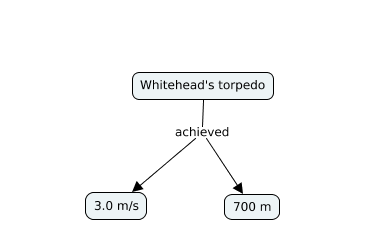
\includegraphics[width=.7\textwidth]{mapa6modi.png}
    \end{figure}
%*----------- notes
    \note[item]{Notes can help you to remember important information. Turn on the notes option.}
\end{frame}
%-
%*----------- SLIDE -------------------------------------------------------------
\begin{frame}[c]{A tropa dos quatro incríveis}
    %\transboxin[duration=1,direction=30]
    A simulação deverá ser desenvolvida com 4 unidades Darwin-OP, comumente esta unidade é utilizada para desafios em competições de robótica.
    \newline

    A tropa será composta por 4 Darwin-OP, e deverá realizar duas missões:
    \begin{itemize}
        \item marchar em forma unida em linha;
        \item realizar corrida de revezamento.
    \end{itemize}

    \begin{figure}
        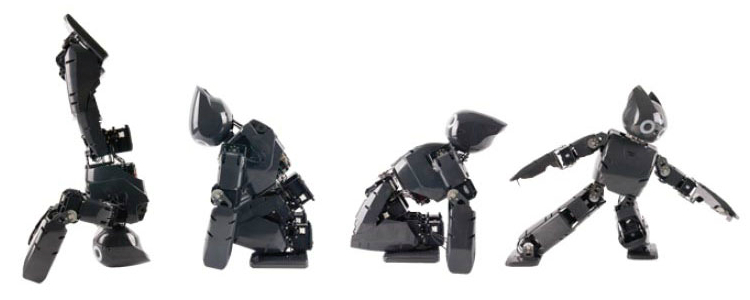
\includegraphics[trim = 0 20 0 50, clip, width=0.8\textwidth]{darwin-op-sequencia}
        %\caption{.}
    \end{figure}
%*----------- notes
    \note[item]{Notes can help you to remember important information. Turn on the notes option.}
\end{frame}
%-
%*----------- SLIDE -------------------------------------------------------------
\begin{frame}[t]{Algumas regras}
    \begin{itemize}
        \item A marcha deverá ser realizada diante de um percurso de 2 metros.
        \item A marcha e a corrida de revezamento deverão serem realizadas numa pista de corrida;
        \item A corrida deverá ser realizada numa pista de 8 metros;
        \item Cada Darwin-OP deverá percorrer 2 metros para realizar o revezamento;
        \item A região de revezamento deverá ser uma área de até 0.4 metros;
        \item O conceito para o revezamento será o de alinhar-se os dois Darwin-OP durante até 15 segundos a uma distância de no máximo 0.2 metros entre ambos, ou seja será considerado passagem de bastão quando os dois Darwin-OP passarem 15 segundos com movimentos sincronizados a uma distância máxima de 0.2 metros dentro da região de revezamento;
        \item A pista de corrida deverá ser considerada analogamente a uma pista real;
        \item A lateral da pista deverá ter lados de 2 metros;
        \item Considerar sempre os critérios de uma corrida de revezamento.
    \end{itemize}
   
    % \begin{columns}[t]
    %     \column{.45\textwidth}
    %         detalhar sistemas em subconjuntos\\
    %         listar possíveis modos de falhas\\
    %         analisar cada modo de falha, juntamente com suas possíveis causas e sintomas
    %     \column{.45\textwidth}
    %         estimar os efeitos de cada modo de falhas\\
    %         estimar a criticidade de cada efeito\\
    %         identificar ações para minimizar falhas
    % \end{columns}
%*----------- notes
    \note[item]{Notes can help you to remember important information. Turn on the notes option.}
\end{frame}
%-
% --------------------------------------Thâmara---------------------------------------------------






% --------------------------------------Alexandre---------------------------------------------------
%*----------- SLIDE -------------------------------------------------------------
\begin{frame}[c]{A pista}
    \begin{figure}
        %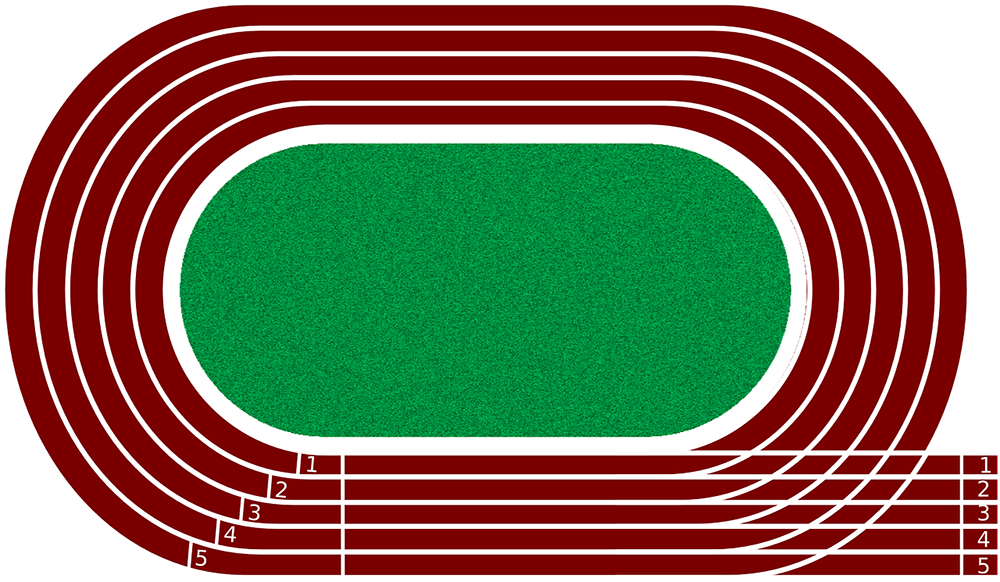
\includegraphics[width=0.7\textwidth]{pista_corrida}
       
        \roundpic[xshift=0cm,yshift=0cm]{3cm}{7cm}{pista_corrida}
          
        \caption{Formato de um pista de corrida.\cite{agostini2007}}
    \end{figure}
%*----------- notes
    \note[item]{Notes can help you to remember important information. Turn on the notes option.}
\end{frame}
%-
%%*----------- SLIDE -------------------------------------------------------------
\begin{frame}[t]{As lideranças das equipes dos Novos Talentos}
    \vspace{0.5cm}
    \begin{columns}
        \column{.01\textwidth}
        \column{.7\textwidth}
            \begin{itemize}
                \item equipe \tikznode{cmark}{RAJA} será liderada por Aziel Freitas
                \item equipe \Circled[outer color=mracula8, inner ysep=8pt]{BORG} será liderada por Mateus Cerqueira.
                \item equipe \Circled[outer color=mracula7, inner ysep=8pt]{BORG} será liderada por Mateus Cerqueira.
                \item equipe \Circled[outer color=mracula9, inner ysep=8pt]{jerotimon} será liderada por Mateus Cerqueira.
                \item equipe TIMON-HM será liderada por Leonardo Lima.
            \end{itemize}
        \column{.29\textwidth}
            
\includegraphics[width=.9\textwidth, trim={10cm 0 10cm 0},clip]{equipe}
    \end{columns}
    \vspace{1cm}
    
    \emph{Para este desafio não será cobrado o relatório técnico, porém o acompanhamento deverá seguir o mesmo ritmo dos desafios anteriores.}

    %add circle on word
    \begin{tikzpicture}[remember picture,overlay]
        \draw[mracula5,very thick] (cmark) circle[x radius=8mm,y radius=4mm]; 
    \end{tikzpicture}
%*----------- notes
    \note[item]{Notes can help you to remember important information. Turn on the notes option.}
\end{frame}
%-
%*----------- SLIDE -------------------------------------------------------------
\begin{frame}[t]{O progresso das equipes}
    Um dos indicadores para o acompanhamento das equipes será o percentual de conclusão geral da equipe.
    O planejamento das atividades deverá seguir a metodologia aplicada no desenvolvimento de projetos de robótica.
    \newline
    %\vspace{0.5cm}
    \begin{table}[ht!]
    \centering
        \caption{PERCENTUAL DE CONCLUSÃO POR EQUIPE}
        \begin{tabular}{|l|c|c|c|c|} \hline
            \textbf{EQUIPE}&\textbf{04/05}&\textbf{11/05}&\textbf{18/05}&\textbf{25/05}\\ \hline
            RAJA & 17\% &32\% & &  \\ \hline
            BORG & 0\% &41\% & &  \\ \hline
            TIMON-HM & 5\% &47\% & &  \\ \hline
        \end{tabular}
    \end{table}
%*----------- notes
    \note[item]{Notes can help you to remember important information. Turn on the notes option.}
\end{frame}
%-
%*----------- SLIDE -------------------------------------------------------------
\begin{frame}[t]{O progresso das equipes}
    Um dos indicadores para o acompanhamento das equipes será o percentual de conclusão geral da equipe.
    O planejamento das atividades deverá seguir a metodologia aplicada no desenvolvimento de projetos de robótica.
    \newline
    %\vspace{0.5cm}
    % \begin{table}[ht!]
    % \centering
    %     \caption{PERCENTUAL DE CONCLUSÃO POR EQUIPE}
    %     \begin{tabular}{|l|c|c|c|c|} \hline
    %         \textbf{EQUIPE}&\textbf{04/05}&\textbf{11/05}&\textbf{18/05}&\textbf{25/05}\\ \hline
    %         RAJA & 17\% &32\% & &  \\ \hline
    %         BORG & 0\% &41\% & &  \\ \hline
    %         TIMON-HM & 5\% &47\% & &  \\ \hline
    %     \end{tabular}
    % \end{table}
%*----------- notes
    \note[item]{Notes can help you to remember important information. Turn on the notes option.}
\end{frame}
%-
%*----------- SLIDE -------------------------------------------------------------
\begin{frame}[t]{O progresso das equipes}
    Um dos indicadores para o acompanhamento das equipes será o percentual de conclusão geral da equipe.
    O planejamento das atividades deverá seguir a metodologia aplicada no desenvolvimento de projetos de robótica.
    \newline
    %\vspace{0.5cm}
    % \begin{table}[ht!]
    % \centering
    %     \caption{PERCENTUAL DE CONCLUSÃO POR EQUIPE}
    %     \begin{tabular}{|l|c|c|c|c|} \hline
    %         \textbf{EQUIPE}&\textbf{04/05}&\textbf{11/05}&\textbf{18/05}&\textbf{25/05}\\ \hline
    %         RAJA & 17\% &32\% & &  \\ \hline
    %         BORG & 0\% &41\% & &  \\ \hline
    %         TIMON-HM & 5\% &47\% & &  \\ \hline
    %     \end{tabular}
    % \end{table}
    
    \url{https://braziliansinrobotics.com/}
%*----------- notes
    \note[item]{Notes can help you to remember important information. Turn on the notes option.}
\end{frame}
%-
%*----------- SLIDE -------------------------------------------------------------
\begin{frame}
    %\transdissolve[duration=0.5]
    %\hspace*{-1cm}
    \begin{columns}
        %\column{.01\textwidth}
        \column{0.4\textwidth}
            ~\hfill
            \vbox{}\vskip-1.4ex%
            \begin{beamercolorbox}[sep=8em, colsep*=18pt, center, wd=\textwidth, ht=\paperheight]{title page header}%
                \begin{center}
                    %\textbf{\huge{\newline}}\pa
                    \textbf{\huge{VISÃO}}\par
                    \vspace*{0.3cm}
                    \textbf{\huge{FUTURA}}\par
                    \vspace*{0.3cm}
                    \textbf{\huge{AUVs}}
                \end{center}
            \end{beamercolorbox}%
        \hfill\hfill
        \column{.05\textwidth} 
        \column{.6\textwidth}
        %\vspace*{cm}
            \begin{itemize}
                \item Estão em uma fase de aceitação
                \item Há uma tendência de crescimento em nível comercial
                \item Os custos em operações de pesquisas em águas profundas podem ser reduzidas em 40\% a 60\%
            \end{itemize}
        \vspace*{2cm}
    \end{columns}
  
 %*----------- notes__
    \note[item]{Notes can help you to remember important information. Turn on the notes option.}
\end{frame}
%-

%----------------------------------------------------SLIDE------------------
 \begin{frame}[t, allowframebreaks]{References}
 %\frametitle{References}
%\begin{frame}{Reference}
    %\transboxin[duration=1,direction=30]

    % \begin{bibunit}[plain]
    % \cite{guangyi2018research}.
    % %\cite{kanakia2012}
    % %\cite{agostini2007}
    % %\cite{azuma1997survey}
    % \cite{Buss2005}
  
    % \putbib
    % \end{bibunit}
  
    %\bibliographystyle{IEEEtran}
    %\bibliographystyle{IEEEtranS}
    %\bibliographystyle{IEEEbib}
    \bibliographystyle{abntex2-alf}
    %\bibliographystyle{abntex2-num}
    %\bibliographystyle{abnt-alf}
    \bibliography{bibliography} 
    %\putbib

%*----------- notes
    %\note[item]{Notes can help you to remember important information. Turn on the notes option.}
\end{frame}
%
%-
%*----------- SLIDE-BACKUP ------------------------------------------------------
% \backupbegin
% %
% \begin{frame}{Backup}
%     Test
% %*----------- notes-------------------------------
% \note{Notes can help you to remember important information. Turn on the notes option.}
% \end{frame}
% %-
% \backupend
% %-
%*----------- QUESTIONS ---------------------------------------------------------
\begin{frame}[c,plain]
    \lastpage{
        \begin{center}   
            {\usebeamerfont{title} Questions?}\\[3ex] 
            %\hspace{1.5cm} 
            marco.a.reis@google.com
        \end{center}
    }
    
    %*----------- notes---------------------------------
    \note[item]{Notes can help you to remember important information. Turn on the notes option.}
\end{frame}
%*-------------------------------------------------------------------------------
\end{document}